% Options for packages loaded elsewhere
\PassOptionsToPackage{unicode}{hyperref}
\PassOptionsToPackage{hyphens}{url}
%
\documentclass[
  12pt,
]{article}
\usepackage{amsmath,amssymb}
\usepackage{lmodern}
\usepackage{iftex}
\ifPDFTeX
  \usepackage[T1]{fontenc}
  \usepackage[utf8]{inputenc}
  \usepackage{textcomp} % provide euro and other symbols
\else % if luatex or xetex
  \usepackage{unicode-math}
  \defaultfontfeatures{Scale=MatchLowercase}
  \defaultfontfeatures[\rmfamily]{Ligatures=TeX,Scale=1}
  \setmainfont[]{Times New Roman}
\fi
% Use upquote if available, for straight quotes in verbatim environments
\IfFileExists{upquote.sty}{\usepackage{upquote}}{}
\IfFileExists{microtype.sty}{% use microtype if available
  \usepackage[]{microtype}
  \UseMicrotypeSet[protrusion]{basicmath} % disable protrusion for tt fonts
}{}
\makeatletter
\@ifundefined{KOMAClassName}{% if non-KOMA class
  \IfFileExists{parskip.sty}{%
    \usepackage{parskip}
  }{% else
    \setlength{\parindent}{0pt}
    \setlength{\parskip}{6pt plus 2pt minus 1pt}}
}{% if KOMA class
  \KOMAoptions{parskip=half}}
\makeatother
\usepackage{xcolor}
\IfFileExists{xurl.sty}{\usepackage{xurl}}{} % add URL line breaks if available
\IfFileExists{bookmark.sty}{\usepackage{bookmark}}{\usepackage{hyperref}}
\hypersetup{
  pdftitle={ENV872 course project: Pigs, Poop, and Public Health},
  pdfauthor={Natasha Jacob and Meilin Chan},
  hidelinks,
  pdfcreator={LaTeX via pandoc}}
\urlstyle{same} % disable monospaced font for URLs
\usepackage[margin=2.54cm]{geometry}
\usepackage{longtable,booktabs,array}
\usepackage{calc} % for calculating minipage widths
% Correct order of tables after \paragraph or \subparagraph
\usepackage{etoolbox}
\makeatletter
\patchcmd\longtable{\par}{\if@noskipsec\mbox{}\fi\par}{}{}
\makeatother
% Allow footnotes in longtable head/foot
\IfFileExists{footnotehyper.sty}{\usepackage{footnotehyper}}{\usepackage{footnote}}
\makesavenoteenv{longtable}
\usepackage{graphicx}
\makeatletter
\def\maxwidth{\ifdim\Gin@nat@width>\linewidth\linewidth\else\Gin@nat@width\fi}
\def\maxheight{\ifdim\Gin@nat@height>\textheight\textheight\else\Gin@nat@height\fi}
\makeatother
% Scale images if necessary, so that they will not overflow the page
% margins by default, and it is still possible to overwrite the defaults
% using explicit options in \includegraphics[width, height, ...]{}
\setkeys{Gin}{width=\maxwidth,height=\maxheight,keepaspectratio}
% Set default figure placement to htbp
\makeatletter
\def\fps@figure{htbp}
\makeatother
\setlength{\emergencystretch}{3em} % prevent overfull lines
\providecommand{\tightlist}{%
  \setlength{\itemsep}{0pt}\setlength{\parskip}{0pt}}
\setcounter{secnumdepth}{5}
\ifLuaTeX
  \usepackage{selnolig}  % disable illegal ligatures
\fi

\title{ENV872 course project: Pigs, Poop, and Public Health}
\usepackage{etoolbox}
\makeatletter
\providecommand{\subtitle}[1]{% add subtitle to \maketitle
  \apptocmd{\@title}{\par {\large #1 \par}}{}{}
}
\makeatother
\subtitle{\url{https://github.com/mchan211/ChanJacob_ENV872_EDA_FinalProject}}
\author{Natasha Jacob and Meilin Chan}
\date{}

\begin{document}
\maketitle

\newpage

\hypertarget{table-of-contents}{%
\section{Table of Contents}\label{table-of-contents}}

\begin{itemize}
\tightlist
\item
  List of Tables
\item
  List of Figures
\item
  Introduction
\item
  Rationale and Research Question
\item
  Dataset Information
\item
  Analysis

  \begin{itemize}
  \tightlist
  \item
    Spatial Analysis
  \item
    Visualization Analysis
  \end{itemize}
\item
  Results and Discussion
\item
  Summary and Conclusions
\item
  Resources
\end{itemize}

\newpage

\hypertarget{list-of-tables}{%
\section{List of Tables}\label{list-of-tables}}

\begin{itemize}
\tightlist
\item
  Dataset information
\item
  Counties used in our analysis
\item
  Counties with high populations of hog farms
\end{itemize}

\hypertarget{list-of-figures}{%
\section{List of Figures}\label{list-of-figures}}

\begin{itemize}
\tightlist
\item
  Hog Farm locations in North Carolina
\item
  Counties with High Populations of Hog Farms
\item
  Population Distribution by County (\%)
\item
  Chronic Health Incidence Rates
\item
  Health Accessibility
\item
  Health Risk Indicators
\end{itemize}

\newpage

\hypertarget{introduction}{%
\section{Introduction}\label{introduction}}

\begin{quote}
Hog farming is the practice of raising and breeding domestic pigs mainly
for their meat and skin. Pigs are a popular form of livestock, with more
than one billion pigs butchered each year worldwide, 100 million of them
in the USA. The discharge of waste from hog farms is usually done by
flushing the waste into giant holding ponds called lagoons. The liquid
waste from the lagoons is then sprayed onto the farmers' fields to keep
the lagoons from filling. The result, according to the farms' neighbors,
is stench and insects and decay from dead hogs that are piled into open
containers before they are removed. The EPA and federal politicians have
drafted little to no regulation surrounding CAFOs to safeguard the
environment and human welfare from their effects. Because manure lagoons
are not connected to a moving water supply, there are little to no
regulations surrounding waste disposal. As a result, they are not
considered a serious threat to human or environmental health.
\end{quote}

\hypertarget{rationale-and-research-questions}{%
\section{Rationale and Research
Questions}\label{rationale-and-research-questions}}

\begin{quote}
Our main research question was if NC counties with higher concentration
of hog farms would have higher health disparities compared to counties
with lower hog farm concentrations. NC Hog farms dispose of pig poop by
collecting enormous amounts of pig pools into lagoons and spraying the
liquidy mixture out onto fields. As you can imagine, the fine mist can
travel some distance and has led to strong odors and health impacts of
neighboring communities. We were interested in seeing the distribution
of populations near where hog farms are concentrated as well as if there
were any disparities in health and health access. To research this, we
looked at health and population distribution data for each NC county and
specifically looked at data for counties with the highest concentrations
of hog farms (Bladen, Duplin, Greene, Sampson, Robeson, Wayne) and
comparing them to counties with low concentrations or no hog farms
(Durham - as we are current residents of this county, Beaufort - as this
is part of Duke's community, Martin, Wilson, and Warren). We wanted to
gain a better understanding of the inequities and environmental justice
issues that stem from NC hog farms and pork production economy.
\end{quote}

\newpage

\hypertarget{dataset-information}{%
\section{Dataset Information}\label{dataset-information}}

\begin{quote}
Our core analysis revolves around the use of spatial datasets of NC
counties and hog farm locations, and a dataset containing population
distribution and health data for each NC county.
\end{quote}

\begin{itemize}
\tightlist
\item
  Spatial Data

  \begin{itemize}
  \tightlist
  \item
    cb\_2018\_us\_county\_20m.shp
  \item
    Hog\_Farm\_Locations\_NC1.csv
  \end{itemize}
\item
  Visualization Data

  \begin{itemize}
  \tightlist
  \item
    CountyHogs\_HealthData.csv
  \end{itemize}
\end{itemize}

\begin{longtable}[]{@{}
  >{\centering\arraybackslash}p{(\columnwidth - 2\tabcolsep) * \real{0.5065}}
  >{\centering\arraybackslash}p{(\columnwidth - 2\tabcolsep) * \real{0.4935}}@{}}
\toprule
\begin{minipage}[b]{\linewidth}\centering
Column Name
\end{minipage} & \begin{minipage}[b]{\linewidth}\centering
Description - all per county
\end{minipage} \\
\midrule
\endhead
Population & Total population \\
Child\_Population\_percentage & \% (per county) \\
Elderly\_Population\_percentage & \% (per county) \\
White\_Population\_percentage & \% (per county) \\
Hispanic\_Latinx\_percentage & \% (per county) \\
African\_American\_percentage & \% (per county) \\
American\_Indian\_percentage & \% (per county) \\
Reading\_Proficiency\_percentage & \% literacy rate per county \\
Uninsured\_Adults\_percentage & \% adults w/out health insurance \\
Medicaid\_CHIP\_enrolles\_percentage & \% individ. w/ Medicaid or
CHIP \\
Primary\_Care\_Physicians & Physicians per 10,000 pop. \\
Low\_Birthweight\_percentage & \% of low birth weight occurrences \\
Infant\_Mortality\_Rate & \% rate of infant mortality \\
Cancer\_Incidence & Incidence rates per 100,000 pop. \\
Heart\_Disease & Death rates per 100,000 pop. \\
Poverty\_percentage & \% of pop. living under poverty line \\
Air\_Pollution & avg. daily density of PM (ug/m3) \\
\bottomrule
\end{longtable}

\begin{quote}
Table 1. Table showing description and units of variables used in the
study
\end{quote}

\begin{longtable}[]{@{}
  >{\centering\arraybackslash}p{(\columnwidth - 2\tabcolsep) * \real{0.5065}}
  >{\centering\arraybackslash}p{(\columnwidth - 2\tabcolsep) * \real{0.4935}}@{}}
\toprule
\begin{minipage}[b]{\linewidth}\centering
High density
\end{minipage} & \begin{minipage}[b]{\linewidth}\centering
Low density
\end{minipage} \\
\midrule
\endhead
Bladen & Wilson \\
Duplin & Warren \\
Greene & Martin \\
Robeson & Beaufort \\
Sampson & Durham \\
Wayne & \\
\bottomrule
\end{longtable}

\begin{quote}
Table 2. Table showing North Carolina counties used in the study -
counties with high and low densities of hog farms in North Carolina
\end{quote}

\begin{center}\rule{0.5\linewidth}{0.5pt}\end{center}

\textbf{Data Wrangling}

The file was first converted from a .xlsx format to a .csv format since
the csv file was found to be more compatible with the functions we used
in R. A detailed explanation of the data wrangling process can be found
below:

\begin{itemize}
\tightlist
\item
  Select and de-select functions were used to remove rows and columns
  containing weblinks and other metadata
\item
  A piped statement was used to select the counties of interest and
  rename the columns
\item
  Transpose function was used to interchange data present in rows and
  columns (x,y) to for easier visualization
\item
  A piped statement was used to rename column names due to the use of
  the `Transpose' function which altered the column names
\item
  A piped statement with the `gsub' function was used to remove `\%'
  characters from values
\end{itemize}

\newpage

\newpage

\hypertarget{data-analysis}{%
\section{Data Analysis}\label{data-analysis}}

\hypertarget{spatial-analysis}{%
\subsection{Spatial Analysis}\label{spatial-analysis}}

\textbf{Hog Farms in North Carolina}

\begin{flushleft}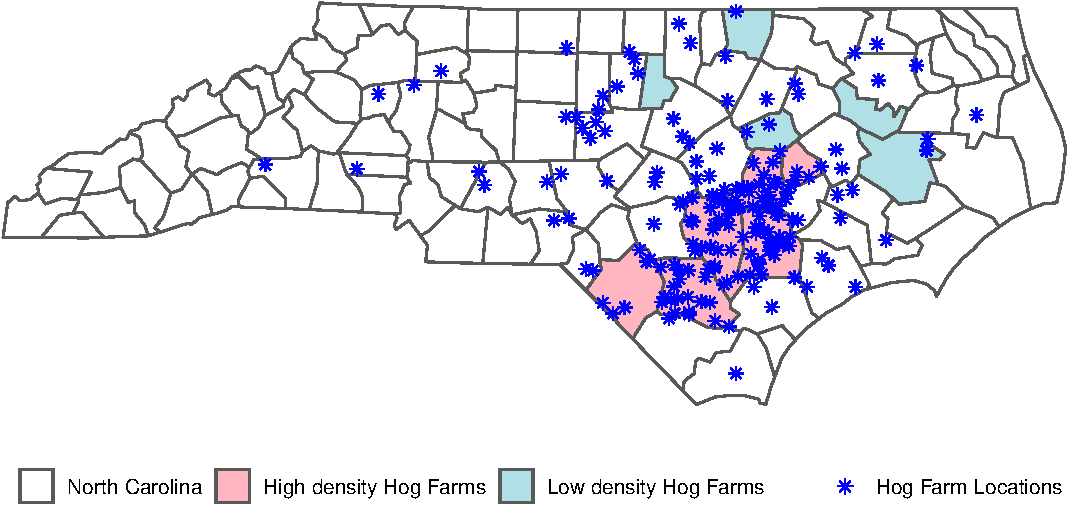
\includegraphics{JacobChan_FinalProject_HogFarms_files/figure-latex/spatial-1} \end{flushleft}

\begin{quote}
Figure 1. Map showing spatial extent of Hog Farm sites located in North
Carolina
\end{quote}

\newpage

\textbf{NC counties with high populations of Hog Farms}

\begin{center}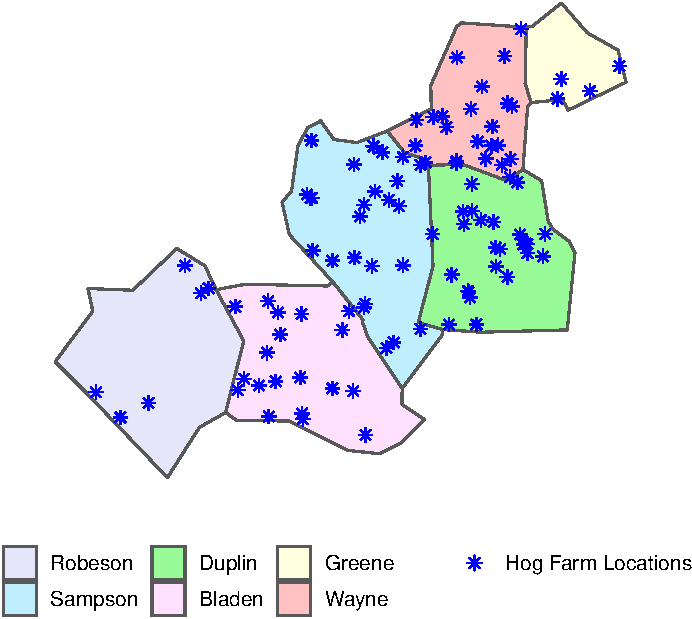
\includegraphics{JacobChan_FinalProject_HogFarms_files/figure-latex/unnamed-chunk-3-1} \end{center}

\begin{quote}
Figure 2. Subset map showing counties with high hog farm density in
North Carolina
\end{quote}

\newpage

\hypertarget{visualization-analysis}{%
\subsection{Visualization Analysis}\label{visualization-analysis}}

\textbf{Population distribution by county (\%)}

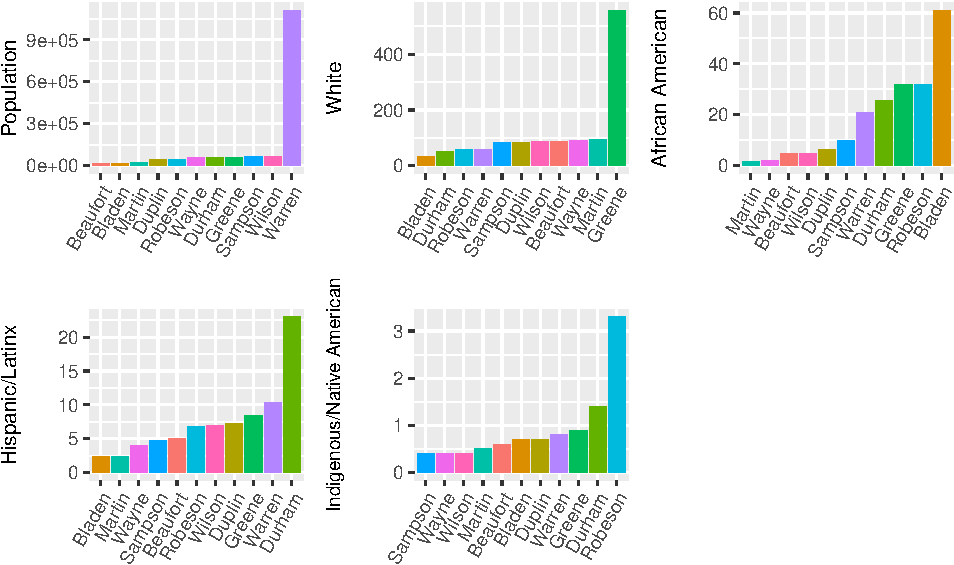
\includegraphics{JacobChan_FinalProject_HogFarms_files/figure-latex/pop final-1.pdf}

\begin{quote}
Figure 3. Population Distribution by County (\%)
\end{quote}

\newpage

\textbf{Chronic Health Incidence Rates}

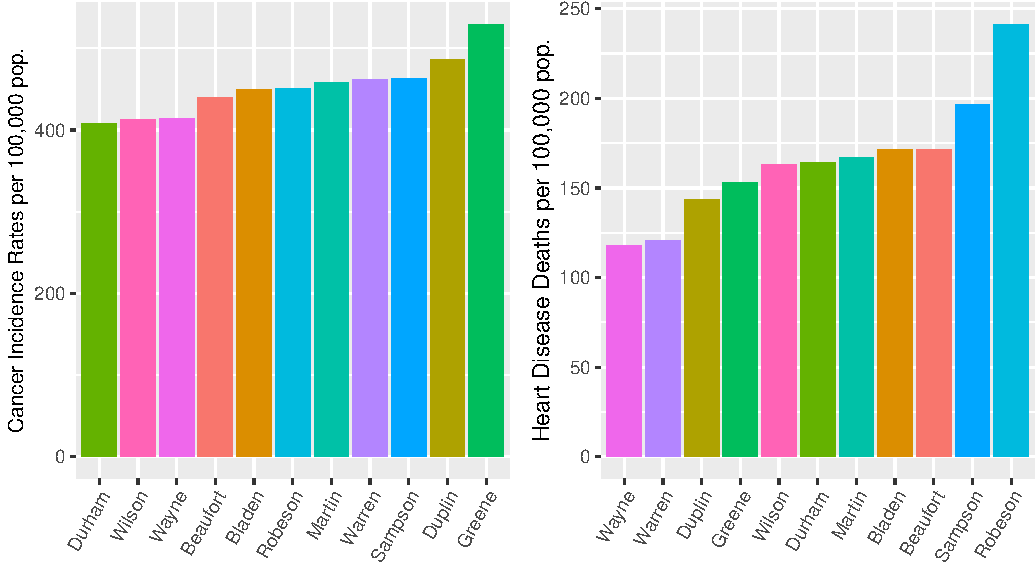
\includegraphics{JacobChan_FinalProject_HogFarms_files/figure-latex/disease final-1.pdf}

\begin{quote}
Figure 4. Chronic Health Incidence Rates
\end{quote}

\newpage

\textbf{Health Risk Indicators}

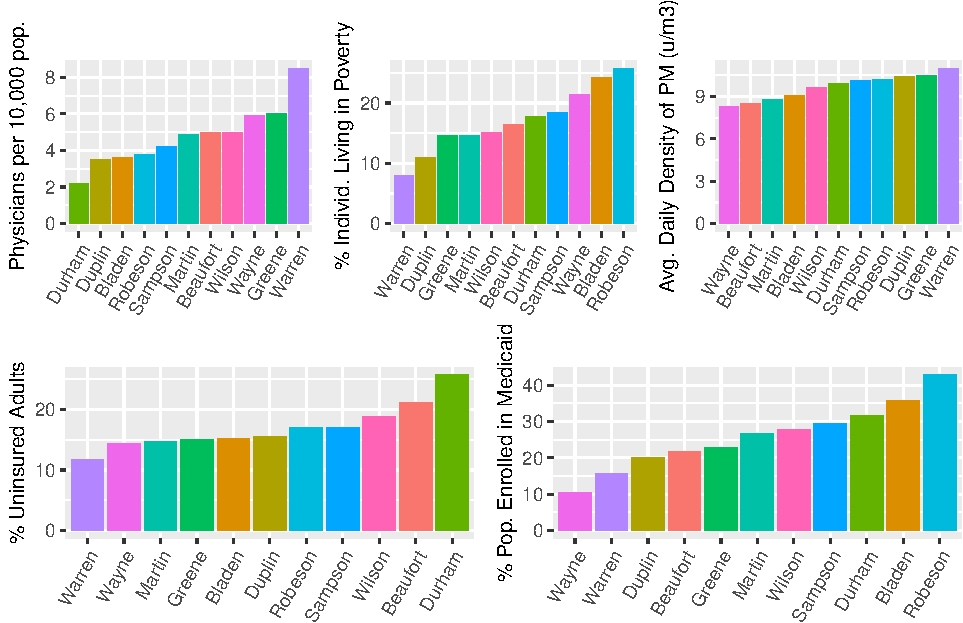
\includegraphics{JacobChan_FinalProject_HogFarms_files/figure-latex/final health-1.pdf}

\begin{quote}
Figure 5. Health Risk Indicators
\end{quote}

\newpage

\textbf{Infant Health Disparities}

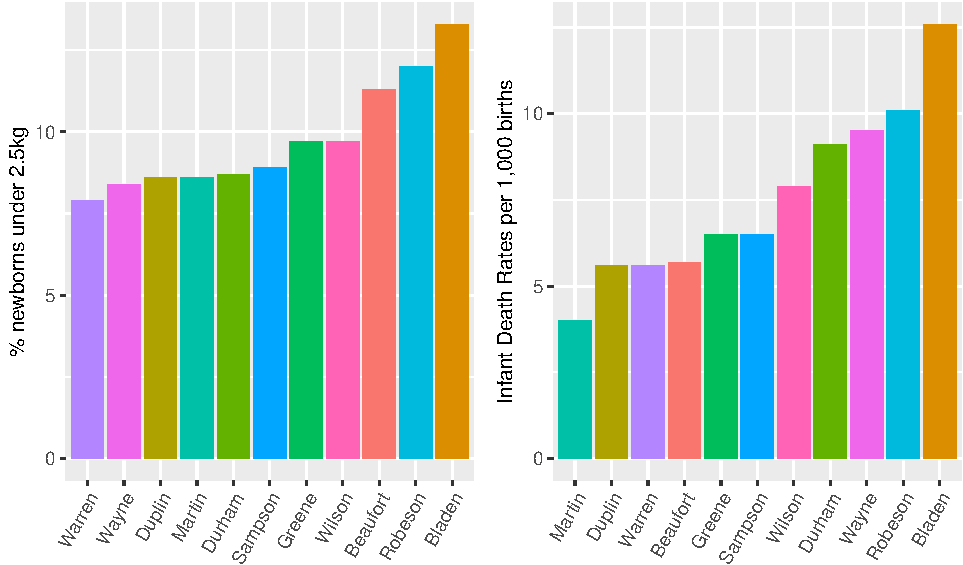
\includegraphics{JacobChan_FinalProject_HogFarms_files/figure-latex/final infant-1.pdf}

\begin{quote}
Figure 6. Infant Health Disparities
\end{quote}

\newpage

\textbf{Vulnerable Populations}

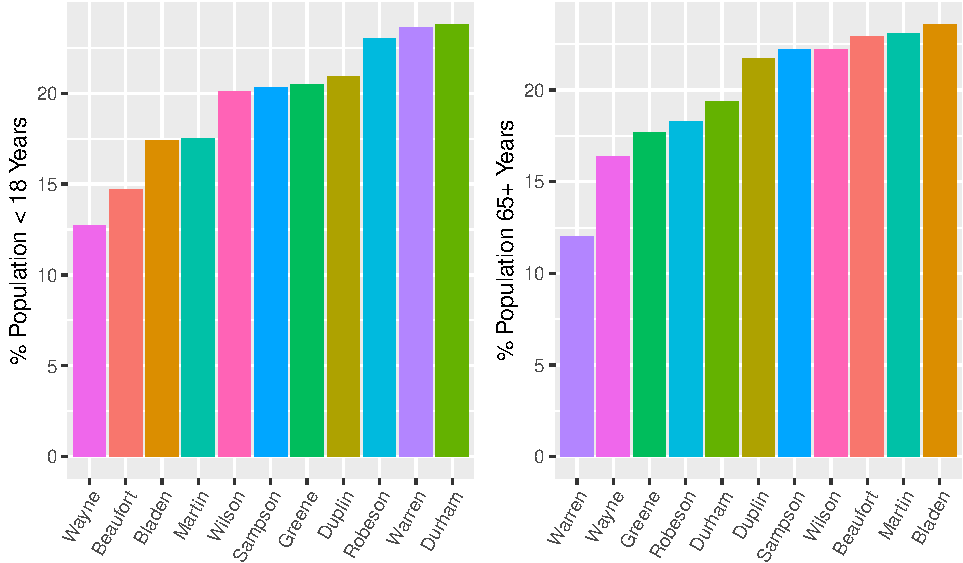
\includegraphics{JacobChan_FinalProject_HogFarms_files/figure-latex/vulnerable final-1.pdf}

\begin{quote}
Figure 7. Vulnerable Populations
\end{quote}

\newpage

\hypertarget{results-and-discussion}{%
\section{Results and Discussion}\label{results-and-discussion}}

\textbf{Question 1: Which NC counties have the highest concentration of
hog farms?}

\begin{quote}
Counties with the highest concentration of hog farms in North Carolina
are Bladen, Duplin, Greene, Robeson, Sampson and Wayne (Table 2).
\end{quote}

\begin{longtable}[]{@{}cc@{}}
\toprule
County & Number of Hog Farms \\
\midrule
\endhead
Sampson & 28 \\
Duplin & 25 \\
Bladen & 19 \\
Robeson & 6 \\
Greene & 4 \\
\bottomrule
\end{longtable}

\begin{quote}
Table 2: NC counties with high density hog farms
\end{quote}

\textbf{Question 2: Are hog farms more prevelant in communities with
higher BIPOC populations?}

\begin{quote}
Counties with higher concentrations of hog farms tend to have a higher
distribution of Hispanic/Latinx and Native American communities compared
to counties with low concentrations of or no hog farms (Figure 3). In
particular, Robeson county has the highest proportion of Native American
individuals compared to all the other counties we analyzed. Sampson and
Duplin have the highest number of hog farms compared to all the counties
we identified, and also has the highest proportion of Hispanic/Latinx
individuals compared to the counties we analyzed.
\end{quote}

\textbf{Question 3: What health inequities are most prevalent in
counties with high concentrations of hog farms?}

\begin{quote}
Counties with high concentrations of hog farms tended to have lower
number of physicians per 10,000 people compared to the other counties we
observed (Figure 5). Further, these counties also had higher \% of
adults without health insurance. Robeson county, which also had the
highest distribution of Native American individuals, also had the
highest \% of its population living in poverty (Figure 5). Counties with
higher concentrations of hog farms also had slightly higher air PM
density measurements - it should be noted that Durham is considered
metropolitan compared to the other analyzed counties and thus would have
a higher average density of PM. The counties with the highest
concentrations of hog farms in particular (Sampson, Duplin) has a
population where a quarter is under 18 years old which is a population
vulnerable to environmental health impacts (Figure 7).
\end{quote}

\newpage

\hypertarget{summary-and-conclusions}{%
\section{Summary and Conclusions}\label{summary-and-conclusions}}

\begin{quote}
Our analysis was just a surface level look at potential connections
between hog farm location in NC, BIPOC communities, and health
disparities. From our visualizations, we see that higher concentrations
of hog farms tend to be in counties with higher distributions of
Hispanic/Latinx and Native American communities compared to counties
with low or no hog farms. Further, communities with higher
concentrations of hog farms also tended to have lower numbers of
available physicians per population size, higher \% of adults without
health insurance, higher average daily density PM measurements, and
higher \% population of children (under 18 years old). Although our
analysis did not find strong relationships between counties with high
concentrations of hog farms and public health impacts on chronic
diseases and infant health, it is possible there are specific health
impacts that are unreported. Our data set did not provide data on
respiratory health or other less deathly health impacts (ie: headaches,
nausea, etc.) that individuals living near hog farms could be
experiencing more frequently.
\end{quote}

\begin{quote}
Future studies could dig further into the impact of hog farm feces
disposal methods on air quality and water quality of Wayne, Bladen,
Greene, Robeson, Sampson, and Duplin counties. With air quality, a study
could measure and visualize daily air quality measurements and see if
there are any increases in PM specifically during periods where the
lagoon feces mixture is sprayed into the air. One could also look into
if there are any unreported health impacts due to inaccessability to
health care in counties with high concentrations of hog farms (ie: no
health insurance, low number of physicians compared to population).
\end{quote}

\newpage

\hypertarget{references}{%
\section{References}\label{references}}

\begin{itemize}
\tightlist
\item
  {[}Environmental Working Group Map - Distribution of Animal
  Agriculture Farms{]}
  \url{https://www.ewg.org/interactive-maps/2020-fields-of-filth/map/}
\item
  {[}NC Farms and Floodplains{]}
  \url{https://sites.tufts.edu/gis/files/2017/06/Moore_Emily_UEP232_2016.pdf}
\item
  {[}Democracy Now! Video on NC Hog Farms{]}
  \url{https://www.youtube.com/watch?v=eyAFNV4Afgw}
\item
  {[}Cartographic Boundary File{]}
  \url{https://www.arcgis.com/sharing/rest/content/items/05f6d4797e2a428d96c15aba40088159/info/metadata/metadata.xml?format=default\&output=html}
\item
  {[}Locations of Hog Farms in North Carolina{]}
  \url{https://www.google.com/maps/search/hog+farms+in+north+carolina/@35.2918991,-79.6807785,8z/data=!3m1!4b1}
\item
  {[}NC Health News{]}
  \url{https://www.northcarolinahealthnews.org/2020/12/04/neighbors-of-hog-farms-say-recent-appeals-court-ruling-gives-them-hope/}
\item
  {[}Phantom Buster{]} \url{https://phantombuster.com/}
\item
  {[}Environmental Health and impacts of pig farming{]}
  \url{https://en.wikipedia.org/wiki/Pig_farming\#Environmental_and_health_impacts}
\end{itemize}

\end{document}
